%%%%%%%%%%%%%%%%%%%%%%%%%%%%%%%%%% PREAMBLE %%%%%%%%%%%%%%%%%%%%%%%%%%%%%%%%%%%%

\documentclass{uvamscse}	% UvA thesis class

% numeric citations, name/title/year sorting
%\usepackage[backend=biber, style=alphabetic, citestyle=alphabetic, sorting=nty]{biblatex}

\usepackage{tikz}
\usepackage{amsmath}
\usepackage{amssymb}
\usepackage[linesnumbered,ruled]{algorithm2e}
\usetikzlibrary{positioning}

% program listings environment, see uvamscse.cls
\usepackage{listings}

\lstdefinelanguage{sdf}{%
  numbers=none,
  morekeywords={module,imports,exports,sorts,context,lexical,free,syntax,==,=,+,-,left,cons,prefer,avoid,bracket},
  columns=flexible,
  morestring=[b]",
  basicstyle=\footnotesize\mdseries,
  literate={->}{{\,\,$\to$\,\,}}1
}

\lstdefinelanguage{dcg}{%
  numbers=none,
  morekeywords={},
  morestring=[b]",
  basicstyle=\footnotesize\mdseries,
  columns=flexible,
}

\lstdefinelanguage{prolog},
  literate={:-}{{\,$\Leftarrow$\,\,}}1 {-->}{{$\to$\,}}1
}

\lstdefinestyle{mono}{
  basicstyle=\footnotesize\ttfamily
}

\lstset{%
  frame=none,
  xleftmargin=2pt,
  stepnumber=1,
  numbers=left,
  numbersep=7pt,
  numberstyle=\ttfamily\scriptsize\color[gray]{0.3},
  belowcaptionskip=\bigskipamount,
  captionpos=b,
%  escapeinside={*'}{'*},
  % language=fl,
  tabsize=2,
  emphstyle={\bf},
  stringstyle=\itshape,
  showspaces=false,
  keywordstyle=\bfseries\rmfamily,
  columns=flexible,
  basicstyle=\small\mdseries,
  showstringspaces=false,
}

\newcommand{\cmd}[1]{\texttt{$\backslash$#1}}

\title{Detecting Online Conversations Going Viral}
\coverpic[250pt]{figures/Buzzcapture_thunder.png}
\subtitle{Time-series aware evaluation of change detection algorithms}
\date{Spring 2017}

\author{Matt Chapman}
\authemail{matthew.chapman@student.uva.nl}
\host{Buzzcapture International, \url{http://www.buzzcapture.com}}
\supervisor{Evangelos Kanoulas, Universiteit van Amsterdam}

\abstract{
	\todo[inline]{Write abstract}
}

\newlength\mylen
\newcommand\myinput[1]{%
  \settowidth\mylen{\KwIn{}}%
  \setlength\hangindent{\mylen}%
  \hspace*{\mylen}#1\\}

\begin{document}
\nocite{*}
\maketitle

%%%%%%%%%%%%%%%%%%%%%%%%%%%%%%%%%%%%%%%%%%%%%%%%%%%%%%%%%%%%%%%%%%%%%%%%%%%%%%%%

\chapter{Problem Statement \& Motivation}

\section{Problem Statement}
\label{Problem Statement}

When asserting the veracity of an approach to a particular problem in software engineering, this is almost always achieved by utilising some sort of metric or measure. To give an example, when evaluating the quality of some new piece of software, this could be done through calculating measures such as McCabe Complexity \todo{cite} or unit test coverage.

The problem of detecting change points in a data stream is no different. There exists within this field a number of metrics that may be used to prove the accuracy and effectiveness of a given approach, and these often fall into one of three categories: binary classification (e.g. F1 score), clustering (e.g. BCubed, or the Rand Index), or information retrieval (e.g. TREC retrieval score)\todo{cite this}.

Being that there are myriad ways to detect change points in a data stream, it is necessary to implement the application of some evaluation measure to back up an assertion that, for example, approach \emph{A} is better than approach \emph{B} for some data set $y_s$. The application of these measures can, in some cases, result in more questions than answers, especially in situations where two different measures may disagree with the results of the aforementioned approaches \emph{A} and \emph{B}.

However, for the number of change point detection methods that exist, there is an almost equal number of ways to evaluate the results of the methods. There is little agreement between researchers on the `correct' method to use, and as this research will show, there are problems that exist when utilising measures that have generally been widely accepted for this purpose.

Outside of the `normal' applications of change point detection (for example, spotting the onset of `storm seasons' in oceanographic data \todo{cite} or the detection of past changes in the valuation of a currency, such as BitCoin \todo{cite}, there is also an application for change point detection as an `event detection' mechanism, when applied to data such as that sourced from online social media platforms.

There exists methods of event detection in social media data utilising approaches such as term frequency counting, lexicon-based recognition and context-free-grammar algorithms \todo{cite yordi}. However, these approaches rely on (sometimes computationally expensive) analysis of the content of messages being posted on social media platforms. Being that change point detection (and especially \emph{online} change point detection algorithms can be utilised for the detection of past events, it stands to reason that these algorithms can also be utilised for event detection when applied to pre-computed data such as conversation volume or reach of a particular conversation. There certainly exists a requirement in the field of online reputation management to be able to inform businesses (in a timely manner) that a spike in conversation volume is occurring, and thus they may need to carry out some action to mitigate reputational damage if the conversation sentiment is negative.

Therefore, this thesis intends to answer the following research questions:

\begin{description}
	\item[RQ1] Are existing change point detection algorithms effective at detecting changes/events in social media data in a timely fashion?
	\item[RQ2] Are measures not specifically defined for the purpose of change detection evaluation effective in this domain?
	\item[RQ3] Do the aforementioned measures agree with by-eye analysis of results from change detection methods?
	\item[RQ4] If existing measures are deficient in some way, what would an `ideal' measure look like?\todo{reword}
\end{description}

From these research questions, the following sub-questions have been formulated:

\begin{description}
    \item[SQ1.1] Which algorithm, out of those being analysed, performs the `best' when applied against real world data?
    \item[SQ2.1] In what way do established measures fail to behave correctly?
    \item[SQ2.2] Which evaluation measure provides the best evaluation, given the functional requirements set forth by the host organisation?
\end{description}

\improvement[inline]{this needs expansion, I think}

\section{Motivation}

This particular research is motivated specifically by the online reputation management sector. The business hosting this research project (Buzzcapture International [\url{http://www.buzzcapture.com}]) is a Dutch consultancy that provides online reputation management services to other businesses throughout Europe. Chief among these services is the BrandMonitor application, which, among other features, provides a rudimentary notification system for clients that is triggered once there is an absolute increase in conversation volume (conversation volume being defined as the number of tweets relevant to the client over a given time period).

Buzzcapture made a project available to students of the Universiteit van Amsterdam, wherein they would provide a method for more effectively providing these notifications, based on more than just an arbitrary threshold on conversation volume or some other computed metric. Upon accepting this project, research was carried out into the field of change detection algorithms, during which it was found that there was not a \emph{single} accepted approach for evaluating measures. Indeed, for every publication that described some novel change point detection algorithm, there was a slightly different approach for evaluating it, and proving the veracity of algorithm in a certain situation. Most publications made use of some sort of binary classification measure, while others had small variations on that theme, providing additional takes on the binary classification approach using methods such as \emph{Receiver Operating Characteristic} curves. Additionally, there were publications that made use of clustering measures, calculated using a segmentation of the time series based on computed change points. \todo{cite}

It is the intention of this thesis to not only answer the research questions set out in \autoref{Problem Statement}, but also to provide a robust recommendation and working prototype of a change detection methodology which could then eventually be implemented into the Brand Monitor tool to supply timely and relevant notifications to clients when a conversation concerning their brand exhibits a change in behaviour or otherwise `goes viral'.

%%%%%%%%%%%%%%%%%%%%%%%%%%%%%%%%%%%%%%%%%%%%%%%%%%%%%%%%%%%%%%%%%%%%%%%%%%%%%%%%

\chapter{Research Method}
\label{Research Method}

\section{Introduction}

The purpose of this thesis is twofold: firstly, to conduct a meta analysis of evaluation measures, and how they perform in the domain of change point detection problems. Being that these measures are metrics designed for other problems that are not necessarily change point detection, it stands to reason that there are perhaps situations where families of metrics will disagree with each-other, or disagree with by-eye evaluation by domain experts. The second purpose is to evaluate the veracity of a number of existing change point detection algorithms when they are applied to data from social media.

This thesis consists of two distinct parts:

\begin{itemize}
  \item Meta-analysis of evaluation measures, fulfilling RQ2 and associated sub-questions.
  \item Application of change detection approaches to real world data and evaluation based on requirements elicitation and evaluation measures.
\end{itemize}

\section{Evaluation Pipeline Construction}

This thesis will analyse three different change detection algorithms: \emph{Pruned Exact Linear Time}\todo{cite}, \emph{Binary Segmentation}\todo{cite} and \emph{Segment Neighbourhoods}\todo{cite}. These will be referred to as \emph{PELT}, \emph{BinSeg} and \emph{SegNeigh} respectively. The algorithms will be briefly discussed in this thesis, along with the chosen critical values such as \emph{minimum segment length}, \emph{penalty scoring} and \emph{assumed underlying distribution}.

The algorithms will then be applied to a collection of datasets falling into two categories: real-world conversation volume data taken from Twitter, and simulated data generated according to certain constraints which will also be discussed here.

The results provided by each technique will then be evaluated according to the following measures: Precision, Recall, F1 score, Rand Index, Adjusted Rand Index, Bcubed Precision, Bcubed Recall and Bcubed F-Score. A meta-analysis will take place to evaluate the effectiveness of these methods when compared with each other and by-eye analysis from social media domain experts.\todo{maybe not}

The method of evaluating the approaches will be developed using a combination of Python and \textsf{R}. \textsf{R} is a combined language and environment created for the purpose of statistical computing \cite{RCoreTeam2017}.

Python is being utilised also due to the availability of relevant software packages for the purposes of evaluation measure calculation.

\subsection{Calculation of Changepoint Locations}

\texttt{changepoint} is a powerful R package that provides a number of different change detection algorithms, along with various approaches to penalty values. \texttt{changepoint} offers change detection in mean, variance and combinations of the two, using the AMOC, PELT, Binary Segmentation and Segment Neighbourhood algorithms\todo{cite these}.

\texttt{Changepoint} was developed by Rebecca Killick and Idris A. Eckley\todo{cite} and is provided free of charge under the GNU general public license \cite{Killick2014}.

\subsection{Calculation of Evaluation Measures}

%The \texttt{ROCR} package in \textsf{R} is being utilised for the calculation of Precision, Recall and F1 scores when treating change detection as a classification problem. \texttt{ROCR} provides a number of functions, and is primarily developed for plotting two different performance measures against each other for the purposes of classification evaluation given a cut-off parameter. \texttt{ROCR} was developed by Tobias Sing et. al. and is provided free of charge under a GPL license\todo{cite}

For the calculation of Precision, Recall and F1 Score, the \textsf{R} package \texttt{caret} is being utilised. \texttt{caret} is an acronym for `Classification and Regression Training, and provides a number of tools for data manipulation, model creation and tuning, and performance measurements. Through the use of this package, it is possible to generate a \emph{confusion matrix} based on algorithm output, and generate various performance measures based upon this. \texttt{caret} was written by Max Kuhn, and is provided free of charge under the GPL license. \todo{cite}

For the calculation of the Rand Index and Adjusted Rand Index the \textsf{R} package \texttt{phyclust} is being used. This package was developed by Wei-Chen Chen, for the purposes of providing a phyloclustering implementation. While this approach is not something being examined in this thesis, the package does provide an implementation of the Rand Index and Adjusted Rand Index metrics, which are relevant to this research. This package is also provided free of charge under the GPL license.\todo{cite}

Calculating the BCubed precision, recall and f-score metrics is being carried out in Python, using the \texttt{python-bcubed} project. This is a small utility library for the calculation of BCubed metrics, developed by Hugo Hromic and provided under the MIT license.\todo{cite} In order to interface with this library via \textsf{R}, the package \texttt{rPython} is being used. This package provides functionality for running Python code and retrieving results in \textsf{R}, and was developed by Carlos J. Gil Bellosta. It is provided under a GPL-2 license.\todo{cite}

Additionally, the \texttt{ROCR} package was utilised during the research phase of this project to generate Receiver Operating Characteristic (ROC) curves - a method used by some publications to evaluate change point detection methods. While ROC curves are not being utilised to produce the results published in this thesis, it was nonetheless an important part of the research, and provided useful insights into binary classification as a field and as a method of evaluation. \texttt{ROCR} was developed by Tobias Sing et. al. and is provided free of charge under a GPL license. \todo{cite}

\section{Measures Meta-Analysis}
\label{meta analysis explainer}

The experiments hereunder were developed to fulfil the requirement to answer research question 2, and it's associated sub-questions:

\begin{itemize}
    \item Are measures not specifically defined for the purpose of change detection evaluation effective in this domain?
    \begin{itemize}
        \item In what way do established measures fail to behave correctly?
        \item Which evaluation measure provides the best evaluation, given the functional requirements set forth by the host organisation?
    \end{itemize}
\end{itemize}

The research questions above are to be answered using a series of experiments carried out using simulated data and algorithms. The experiments intend to test the following criteria:

\begin{enumerate}
    \item Dependence on sample size (otherwise referred to here as time series length)
    \item Impact of data preceding a known change point and its detection
    \item Impact of data following a known change point and its detection
    \item Ability to provide a temporal penalty for late, early or exact detections
    \item Ability to penalise correctly for false positives
    \item Ability to penalise correctly for false negatives
\end{enumerate}

\subsection{Experiment Listings}

For each experiment description, the sample size (otherwise known as time series length) is denoted by $n$, the true change point in the time series is denoted as $\tau_n$ and any `detected' change points are denoted by $\tau'_{n}$. For each experiment, the changing variable (the iterator in the \textsf{R} source code) is denoted as $i$.

\subsubsection{Experiment 1}

This experiment involves increasing the `head' (sample size prior to a single known change point) of a time series, prepending to and thus lengthening the time series. The time series contains a single known change point, and a detected change point provided by a pseudo-algorithm is detected 6 points before the true change point.

For each prepended point, all of the evaluation metrics are calculated and plotted. The experiment evaluates both criteria 1 and 2.

The experiment runs such that $n = 55$ on commencement, and $n = 500$ upon completion, with each iteration adding a single data point such that $i = 445$. For each iteration, $\tau = i + 1$ and $\tau' = n - 4$.


\subsubsection{Experiment 2}

This experiment involves increasing the `tail' (sample size after a single known change point) of a time series, appending to and thus lengthening the time series. The time series contains a single known change point and a detected change point provided by a pseudo-algorithm is detected 4 points before the true change point.

For each appended point, all of the evaluation metrics are calculated and plotted. The experiment evaluates both criteria 1 and 3.

The experiment runs such that $n=55$ on commencement, and $n=550$ upon completion, with each iteration adding a single data point such that $i$ runs from 2 to 500. For each iteration, $\tau = 51$ and $\tau' = 45$.


\subsubsection{Experiment 3}

This experiment involves moving a known change point and a computed change point through a fixed length time series. The time series contains a single known change point and a detected change point provided by a pseudo-algorithm that is detected 5 data points before the true change point.

For each iteration of the experiment, all of the evaluation metrics are calculated and plotted. The experiment evaluates both criteria 1 and 2.

The experiment runs such that $n$ is constant at $n=501$. For each iteration, $\tau = i$ and $\tau' = i - 3$, for values of $i$ from 5 to 500.


\subsubsection{Experiment 4}

This experiment involves moving a detected change point provided by a `pseudo-algorithm' through a time series of fixed length, thus evaluating the ability of a measure to provide a temporal penalty for late, early, or exact detections.

For each iteration of the experiment, all of the evaluation metrics are calculated and plotted. The experiment evaluates criterion 4.

The experiment runs such that $n$ is constant at $n=500$. For each iteration $\tau = 51$ and $\tau' = i$, where $i = 51$ at the commencement (such that $\tau = \tau'$) and $i = 500$ at completion.



\subsubsection{Experiment 5}

This experiment involves adding `false positive' change point detections to a time series of fixed length with a single known change point location.

For each iteration of the experiment, all of the evaluation metrics are calculated and plotted. The Experiment evaluates criterion 4.

The experiment runs such that $n$ is constant at $n=500$. For each iteration $\tau = 51$ and $\tau' = i$, where $i = 51$ at the commencement of the experiment, $i=55$ at the second iteration, and increases in increments of 5 until $i = 500$. This serves to move the detected change point through the time series, starting at the true change point and progressing to the end of the time series, ending at the final point of the time series.



\subsubsection{Experiment 6}

Removing `false negative' results (by way of explanation, adding correct detections) to a fixed length time series, thus increasing the number of correctly detected change points.



\subsubsection{Experiment 7}

Adding both true change points and detected change points from a `pseudo algorithm' that provides detections $n$ points \todo{check this} to a time series, by appending to it, and thus increasing it's length.

\subsubsection{Experiment 8}

Adding both true change points and detected change points from a `pseudo algorithm' that provides detections $n$ points \todo{check this} to a time series of fixed length.

\subsection{Illustrative Algorithms for Experiments}

\begin{algorithm}
\caption{Experiment to plot the effect of increasing `head' length of a dataset on metrics}
\Begin{
    \ForEach{iteration}{
        Add 1 point to head of data, increasing length\\
        Calculate metrics for current $\tau$, $\tau'$ against time series\\
        Store results
    }
}
\end{algorithm}


\begin{algorithm}
\caption{Experiment to plot the effect of increasing `tail' length of a dataset on metrics}
\Begin{
    \ForEach{iteration}{
        Add 1 point to tail of data, increasing length\\
        Calculate metrics for current $\tau$, $\tau'$ against time series\\
        Store results
    }
}
\end{algorithm}

\begin{algorithm}
\caption{Experiment to plot the effect of increasing `tail' length of a dataset on metrics}
\Begin{
    \ForEach{iteration}{
        Move $\tau$ and $\tau'$ 1 point further in time series\\
        Calculate metrics for current $\tau$, $\tau'$ against time series\\
        Store results
    }
}
\end{algorithm}

\begin{algorithm}
\caption{Experiment to plot the effect of temporal distance between $\tau$ and $\tau'$ on metrics}
\Begin{
    \ForEach{iteration}{
        Leave $\tau$ unchanged\\
        $\tau' \leftarrow \tau' + 1$\\
        Calculate metrics for current $\tau$, $\tau'$ against time series\\
        Store results
    }
}
\end{algorithm}

\begin{algorithm}
\caption{Experiment to plot the effect of increasing the number of false positive detections on metrics}
\Begin{
    \ForEach{iteration}{
        Add 1 additional false positive, such that $\tau'_{n+1} = \tau'_{n} + 5$\\
        Calculate metrics for current $\tau$, $\tau'$ against time series\\
        Store results
    }
}
\end{algorithm}

\begin{algorithm}
\caption{Experiment to plot the effect of decreasing the number of false negative detections on metrics}
\Begin{
    \ForEach{iteration}{
        Add one additional $\tau'$ such that $\tau'_n = \tau_n$\\
        Calculate metrics for current $\tau$, $\tau'$ against time series\\
        Store results
    }
}
\end{algorithm}

\begin{algorithm}
\caption{Experiment to plot the effect of the number of change points on metrics, by appending}
\Begin{

    $new\_point \leftarrow$ time series segment with 1 changepoint

    \ForEach{iteration}{
        Append $new\_point$ to data, increasing length\\
        Add additional $\tau$ at $tau_{new\_point}$\\
        Add additional $\tau'$ at $tau'{new\_point}$\\
        Calculate metrics for current $\tau$, $\tau'$ against time series\\
        Store results
    }
}
\end{algorithm}

\begin{algorithm}
\caption{Experiment to plot the effect of the number of change points on metrics, by adding 1 to slices of the time series \& maintaining constant time series length}
\Begin{
    \ForEach{iteration}{
        Add 1 to next slice of time series\\
        Add $\tau$ and $\tau'$ such that $\tau' = \tau + 2$\\
        Calculate metrics for current $\tau$, $\tau'$ against time series\\
        Store results
    }
}
\end{algorithm}

\section{Comparison of Measures Based Upon Functional Requirements}

As part of the research being carried out, a set of functional requirements are elicited from the host organisation. Based on these functional requirements, a 

\section{Application of Algorithms to Real World Data}

\subsection{Data Preparation}

The experiment is being carried out using conversation volume data taken from Buzzcapture's Brand Monitor application. Brand Monitor harvests tweets via the Twitter API and makes them searchable through a bespoke interface as well as providing a number of useful metrics for reputation management. In order to gain data for this experiment, Social Media Analysts from Buzzcapture were requested to provide query strings for the Brand Monitor application, showing a situation where they feel a client should have been informed of a distinct change in conversation volume. The analysts were then asked to manually annotate the data with the points at which they believe a change point detection algorithm should detect a change. In this way, bias is avoided when establishing the ground truth for the data - the author was not involved in this annotation process other than providing instructions. The result of this exercise is then a set of time series' showing the twitter conversation volume over time for a given brand. This is accompanied by a separate data set containing indices at which changes \emph{should} be detected - thus serving as the ground truth for this part of the experiment.

Once the query strings provided were executed, the corpus of test data included the following data sets:

\begin{itemize}
    \item Dirk
    \item Bol.com
    \item Connexion
    \item DAP
    \item Jumbo
    \item Kamer van Koophandel
    \item Rabobank
    \item Tele2
    \item UWV
    \item Ziggo
\end{itemize}

All data sets were trimmed such that the sample size equals 60 for every set. The sets were exported from the BrandMonitor application in CSV format, with daily conversation volume totals.

\subsection{Execution}

To perform the experiment, an \textsf{R} script is executed that reads the CSV file containing the data points being analysed, and reads them into a data frame object. At this point, the data frame is passed to \texttt{changepoint} method calls, running the following analysis methods:

\begin{itemize}
    \item Mean, using PELT
    \item Mean, using SegNeigh
    \item Mean, using BinSeg
    \item Variance, using PELT
    \item Variance, using SegNeigh
    \item Variance, using BinSeg
    \item Mean \& Variance, using PELT
    \item Mean \& Variance, using SegNeigh
    \item Mean \& Variance using BinSeg
\end{itemize}

Once all of the analysis methods have been executed successfully, the measures are calculated based on a comparison between the computed change points and the manually annotated ground truth. These results are then arranged in a tabular format for analysis and discussion.

\section{Algorithm Configuration}

Change detection is an \emph{unbounded} problem. Left without some system of constraint, the algorithm could theoretically run to infinity. Indeed, one of the algorithms utilised in this research, PELT\todo{citation needed}, when left unbounded, will detect every data point in the time-series as a change point. This result is \textit{technically} correct, but not useful for our purposes. For this reason, the algorithms implement a penalty system, allowing for an optimal number of change points to be detected.

\subsection{Distribution Assumptions}

It is also important to note that many change point detection methods make an assumption about the underlying distribution of the data being analysed. This distribution can be, for example, a normal distribution, poisson 

%%%%%%%%%%%%%%%%%%%%%%%%%%%%%%%%%%%%%%%%%%%%%%%%%%%%%%%%%%%%%%%%%%%%%%%%%%%%%%%%

\chapter{Background \& Context}

Change detection first came about as a quality control measure in manufacturing, and methods within this domain are generally referred to as \emph{control charts}. Since the inception of approaches such as CUSUM that provide the possibility for on-line evaluation of continuous data streams, change detection has grown as a field. With applications such as epidemic detection, online reputation management and infrastructure error detection, change detection is hugely useful both as an academic problem and in production systems of myriad application.

\section{Change Detection Algorithms}

\subsection{Pruned Exact Linear Time}

\begin{algorithm}
\caption{PELT Method for change point detection}
\KwIn{A set of data of the form, $(y_1, y_2, \ldots,y_n)$ where $y_i \in \mathbb{R}$.}
\myinput{A measure of fit $C(.)$ dependent on the data.}
\myinput{A penalty constant $\beta$ which does not depend on the number or location of change points.}
\myinput{A constant $K$}
\end{algorithm}

\section{Evaluation Measures}

As briefly discussed in the introduction to this thesis, there are a number of pre-existing approaches for the evaluation of change detection methods. Here, the measures being evaluated are briefly explained:

\begin{description}
	\item[F1 Score]\unsure{cite this?} This measure is utilised for testing accuracy in problems of binary classification. It considers two different measures, \emph{precision} and \emph{recall}, and takes a harmonic mean of the two measures to compute the final score.
	
	To calculate Precision and Recall, a \emph{confusion matrix} is first constructed to provide values for the total number of true positives, false negatives, false positives and true negatives:
	
	\begin{center}
	    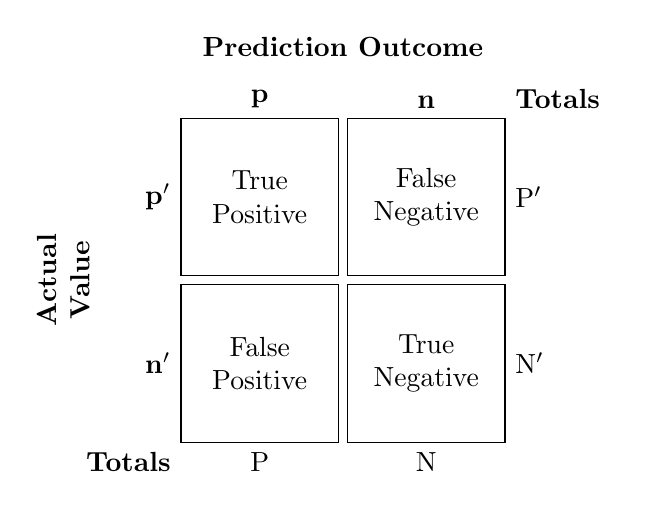
\begin{tikzpicture}[box/.style={draw,rectangle,minimum size=2cm,text width=1.5cm,align=center}]
            \matrix (conmat) [row sep=.1cm,column sep=.1cm] {
            \node (tpos) [box,
               label=left:\( \mathbf{p'} \),
                label=above:\( \mathbf{p} \),
            ] {True \\ Positive};
            &
            \node (fneg) [box,
                label=above:\textbf{n},
                label=above right:\textbf{Totals},
                label=right:\( \mathrm{P}' \)] {False \\ Negative};
            \\
            \node (fpos) [box,
                label=left:\( \mathbf{n'} \),
                label=below left:\textbf{Totals},
                label=below:P] {False \\ Positive};
            &
            \node (tneg) [box,
                label=right:\( \mathrm{N}' \),
                label=below:N] {True \\ Negative};
            \\
            };
    
            \node [rotate=90,left=.05cm of conmat,anchor=center,text width=1.5cm,align=center] {
                \textbf{Actual Value}
            };
            \node [above=.05cm of conmat] {\textbf{Prediction Outcome}};
        \end{tikzpicture}
	\end{center}

	$Recall$ is computed as the number of correct positive results, divided by the number of positive results that should have been detected. $Precision$ is computed as the number of correct positive results divided by the number of all possible positive results:
	
	\begin{eqnarray}
	    Precision = \frac{TP}{TP + FP}\\
	    Recall = \frac{TP}{TP + FN}
	\end{eqnarray}
	
	The F1 score calculation (the harmonic mean of both recall and precision) can be described in general terms as follows:

	\begin{equation}
		F_1 = 2 \cdot \frac{1}{\frac{1}{recall} + \frac{1}{precision}} = 2 \cdot \frac{precision \cdot recall}{precision+recall}
		\label{equ:F1}
	\end{equation}

	As the F1 score is a binary classification measure, it can only be used to test the precision of an algorithm in a single domain, that is, was the change detected or not. Precision, Recall and F1 Score all provide a score $s$ such that $ \{s\in\mathbb{R} \mid 0\leq s \leq 1\} $

	\item[Rand Index] This measure is for computing the similarity between two clusters of data points. It is used for calculating the overall accuracy of a given clustering approach, when compared against a set of ground truth clusters. The Rand Index is defined as:

	\begin{equation}
		R = \frac{a+b}{a+b+c+d}
	\end{equation}
	
	Given a set of data points $S$, partitioned through two different methods, which we shall refer to as $X$ and $Y$. Based on this knowledge the following can be defined:
	
	\begin{itemize}
		\item $a$ = total number of pairs that were partitioned into the \emph{same} subset by both $X$ and $Y$
		\item $b$ = total number of pairs that were partitioned into \emph{different} subsets by both $X$ and $Y$
		\item $c$ = total number of pairs that were partitioned into the \emph{same} subset by $X$ and into a different subset by $Y$
		\item $d$ = total number of pairs that were partitioned into the \emph{same} subset by $Y$ and into a different subset by $X$
	\end{itemize}\todo{reword, wikipedia}
	
	Intuitively, it can be stated that $a+b$ is the total number of agreements between methods $X$ and $Y$, while $c+d$ is the total number of disagreements. This calculation will return $0$ for completely different clusters and $1$ for identical clusters. The Rand Index provides a score $s$ such that $ \{s\in\mathbb{R} \mid 0\leq s \leq 1\} $
	
	\item[Adjusted Rand Index]Similar to the Rand Index, but adjusted to take into account the random chance of pairs being assigned to the same cluster by both approaches being compared. While the Rand Index is suited for comparing a segmentation method against a known-good \emph{oracle} method, the adjusted index is more suited to comparing two differing approaches \cite{Matteson2012}. It is defined as:
	
	\begin{equation}
	    R_{adjusted} = \frac{R - R_{expected}}{R_{max} - R_{expected}}
	\end{equation}
	
	where $R_{expected}$ is defined as the expected Rand Index score for two completely random classifications of the given data\todo{cite, https://arxiv.org/pdf/1306.4933.pdf} and $R_{max}$ is defined as the maximum Rand Index value - generally $1$.
	
	The Adjusted Rand Index provides a score $s$ such that $ \{s\in\mathbb{R} \mid -1\leq s \leq 1\} $. This is different to the score returned by the `basic' Rand Index, in that it is possible for a negative value to be returned.
		
	\item[BCubed] BCubed is similar to the Adjusted Rand Index, in that it is adjusted to be appropriate for all constraints in a clustering problem. It was developed by Bagga and Baldwin\todo{cite} in 1998.
	
	BCubed operates in a similar way to the Recall and Precision classification metrics, in that it computes precision and recall values, before calculating a harmonic mean of the two metrics. BCubed also makes use of an additional \emph{correctness} function defined as follows, where $e$ and $e'$ are equivalent elements in a ground truth and computed clustering respectively, $L$ is a computed label and $C$ is a ground truth category:
	
	\begin{equation}
	\label{eqn:correctness}
	    \text{Correctness}(e,e') = 
	    \begin{cases}
	        1 & \text{iff $L(e) = L(e') \leftrightarrow C(e) = C(e')$}\\
	        0 & \text{otherwise}
	    \end{cases}
	\end{equation}
	
	\autoref{eqn:correctness} can be stated intuitively as returning $1$ if and only if both the ground truth and computed clusterings place the element $e$ into the same cluster, returning $0$ in all other cases.
	
	Precision and Recall can then be calculated as follows:
	
    \begin{align}
    \label{eqn:bcubed-precision}
        \text{Precision} &= Avg_e [Avg_{e' . C(e) = C(e')}[Correctness(e,e')]]\\
        \label{eqn:bcubed-recall}
        \text{Recall} &= Avg_e [Avg_{e' . L(e) = L(e')}[Correctness(e,e')]]
    \end{align}

To obtain the F score, a harmonic mean of Precision and Recall is taken in the same manner as the F1 score for binary classification:

\begin{equation}
    F_{bc} = 2 \cdot \frac{1}{\frac{1}{Recall_{bc}} + \frac{1}{Precision_{bc}}}
\end{equation}

\end{description}

\subsection{Penalty Scores}

Penalty scores operate as a mechanism for optimising an unbounded problem such as the one being addressed here. Haynes et al. define the problem as follows \cite{Haynes2014}: Given time series data points $y_1,\ldots,y_n$, the series will contain $m$ change points such that their locations $\tau_{1:m} = (\tau_1,\ldots,\tau_m)$, where $\{\tau_i \in \mathbb{Z} \mid 1 \leqslant \tau_i \leqslant n-1\}$. $\tau_0$ is assumed to be 0, and $\tau_{m+1}$ is assumed to be $n$. In this way we can state that a given change detection algorithm will split the time series into $m + 1$ segments such that segment $i$ contains the points $y_{(\tau_{i-1}+1):\tau_i} = (y_{\tau_{i-1} + 1},\dots,y_{\tau_i})$. A \emph{cost function} for a segmentation of the data set $y_s$ can be defined as $C = (y_{s+1:t})$. This cost function defines a cost for a given segmentation containing points $y_{s+1:t}$. To illustrate, the cost function $C$, in the context of binary classification, returns a value that increases for an `incorrect' classification and decreases for a `correct' classification.

At this point it can be stated that the \emph{constrained minimisation problem} is as follows:

\begin{equation}
\label{unbounded}
    Q_m(y_{1:n}) = \min_{\tau_{1:m}} \Bigg\{ \sum^{m+1}_{i=1}[C(y_{(\tau_{i - 1} + 1):\tau_i})] \Bigg\}
\end{equation}

\autoref{unbounded} is an equation showing the optimisation problem that change point detection presents. If the equation is taken intuitively, it shows that for a dataset with a \emph{known} number of change points, the segmentation of the data around the change points can be effectively estimated by obtaining the segmentation that returns the minimum cost based on the cost function $C$.

However, the problem being solved by many change detection algorithms involves an unknown number of change points, at unknown locations. In this case we can estimate the following to obtain the number and location of the change points:

\begin{equation}
\label{eqn:penalty}
    \min_{m} \big\{ Q_m(y_{1:n}) + f(m) \big\}
\end{equation}

\autoref{eqn:penalty} includes a \emph{penalty function} $f(m)$ that increases proportionally with the number of change points $m$. Essentially, as the segmentation calculated as $Q_m$ increases in size, so does the result of the penalty function $f(m)$. These two elements are at-odds with each other, presenting a problem that requires optimisation to correctly estimate the number and location of change points in the data set $y_s$. If $f(m)$ increases in a linear fashion with $m$, we can define a \emph{penalised minimisation problem} in the following manner:

\begin{equation}
\label{bounded}
    Q_m(y_{1:n}, \beta) = \min_{m,\tau_{1:m}} \Bigg\{ \sum^{m+1}_{i=1}[C(y_{(\tau_{i - 1} + 1):\tau_i}) + \beta] \Bigg\}
\end{equation}

In this equation, $\beta$ is the penalty function defined previously as $f(m)$.

There are a number of established approaches to calculating penalty values for unbounded problems, chiefly among which are Schwarz Information Criterion (SIC)/Bayesian Information Criterion (BIC), Akaike Information Criterion (AIC) and Hannan-Quinn\todo{cite}. Of these approaches, it is necessary to experiment to find the scheme that produces the `correct' number of change points for a given dataset. The penalty schemes are defined as follows:

\begin{align}
    \text{SIC} &= \ln(n) k - 2 \ln(\hat{L})\\
    \text{AIC} &= 2k - 2 \ln(\hat{L})\\
    \text{HQC} &= -2L_{max} + 2k \ln(\ln(n))
\end{align}

Where $n$ is the total number of observations, $k$ is the number of \emph{free parameters}\footnote{variables that are unable to be predicted by a given model} and $\hat{L}$ is the maximum value of a likelihood function.\todo{reword, wikipedia}

The penalty function returns a value which is represented by $\beta$ in \autoref{bounded}, which then limits the number of possible segmentations returned by $Q$. In this way, varying the penalty function $\beta$ can alter the results given by a change detection algorithm by increasing or decreasing the number of change points detected.

The \texttt{changepoint} package requires the provision of a penalty function for each algorithm, which has been arbitrarily chosen as `Hannan-Quinn' for this research. This does leave an open research question concerning how well each possible penalty function fits the data being evaluated here, but at the time of writing, this falls outside of the scope of this research.\todo{actually, lets do this}

%%%%%%%%%%%%%%%%%%%%%%%%%%%%%%%%%%%%%%%%%%%%%%%%%%%%%%%%%%%%%%%%%%%%%%%%%%%%%%%%

\chapter{Research}

%%%%%%%%%%%%%%%%%%%%%%%%%%%%%%%%%%%%%%%%%%%%%%%%%%%%%%%%%%%%%%%%%%%%%%%%%%%%%%%%

\chapter{Results}

%%%%%%%%%%%%%%%%%%%%%%%%%%%%%%%%%%%%%%%%%%%%%%%%%%%%%%%%%%%%%%%%%%%%%%%%%%%%%%%%

\chapter{Analysis \& Conclusions}

%%%%%%%%%%%%%%%%%%%%%%%%%%%%%%%%%%%%%%%%%%%%%%%%%%%%%%%%%%%%%%%%%%%%%%%%%%%%%%%%

\bibliographystyle{alphaurl}
\bibliography{../Bib/library.bib}

\newpage

\listoftodos[ToDo Notes]

\end{document}
